\documentclass[14pt]{extarticle}
%\usepackage[14pt]{extsizes}

%% подключаем стандарт библиографии
\bibliographystyle{gost71u} 

%% for envirovemt "abstract" in class book
%\newenvironment{abstract}{}{}
%\usepackage{abstract}

%% подключаем преамбулу, в ней содержатся подключение всех необходимых пакетов
%%% Работа с русским языком
\usepackage{cmap}			 % поиск в PDF
\usepackage{mathtext} 		 % русские буквы в формулах
\usepackage[T2A]{fontenc}	 % кодировка
\usepackage[utf8]{inputenc}	 % кодировка исходного текста
\usepackage[russian]{babel}	 % локализация и переносы

%%% Пакеты для работы с математикой
\usepackage{amsmath,amsfonts,amssymb,amsthm,mathtools}
\usepackage{icomma}

%%% Работа с таблицами
\usepackage{array,tabularx,tabulary,booktabs} % Дополнительная работа с таблицами
\usepackage{longtable}  % Длинные таблицы
\usepackage{multirow} % Слияние строк в таблице

%% Номера формул
%\mathtoolsset{showonlyrefs=true} % Показывать номера только у тех формул, на которые есть \eqref{} в тексте.
%\usepackage{leqno}               % Немуреация формул слева

%% Шрифты
\usepackage{euscript}	 % Шрифт Евклид
\usepackage{mathrsfs}    % Красивый матшрифт

%% Поля (геометрия страницы)
\usepackage[left=3cm,right=2cm,top=2cm,bottom=2cm,bindingoffset=0cm]{geometry}

%% Русские списки
\usepackage{enumitem}
\makeatletter
\AddEnumerateCounter{\asbuk}{\russian@alph}{щ}
\makeatother

%%% Работа с картинками
\usepackage{caption}
\RequirePackage{caption}
\DeclareCaptionLabelSeparator{defffis}{ --- }
\captionsetup{justification=centering,labelsep=defffis}
\addto\captionsrussian{\renewcommand{\figurename}{Рисунок}}
\captionsetup{justification=centering} % центрирование подписей к картинкам
\usepackage{graphicx}                  % Для вставки рисунков
\graphicspath{{images/}{images2/}}     % папки с картинками
\setlength\fboxsep{3pt}                % Отступ рамки \fbox{} от рисунка
\setlength\fboxrule{1pt}               % Толщина линий рамки \fbox{}
\usepackage{wrapfig}                   % Обтекание рисунков и таблиц текстом

%%% Работа с таблицами
\usepackage{array,tabularx,tabulary,booktabs} % Дополнительная работа с таблицами
\usepackage{longtable}                        % Длинные таблицы
\usepackage{multirow}                         % Слияние строк в таблице

%% Красная строка
\setlength{\parindent}{2em}

%% Интервалы
\linespread{1}
\usepackage{multirow}

%% TikZ
\usepackage{tikz}
\usetikzlibrary{graphs,graphs.standard}

%% Верхний колонтитул
%\usepackage{fancyhdr}
%\pagestyle{fancy}
%\pagestyle{plain}

% Цвет текста
\usepackage[]{color}
\usepackage{colortbl}

%% Перенос знаков в формулах (по Львовскому)
\newcommand*{\hm}[1]{#1\nobreak\discretionary{}{\hbox{$\mathsurround=0pt #1$}}{}}

%% дополнения
\usepackage{float}   % Добавляет возможность работы с командой [H] которая улучшает расположение на странице
\usepackage{gensymb} % Красивые градусы
\usepackage{caption} % Пакет для подписей к рисункам, в частности, для работы caption*

% подключаем hyperref (для ссылок внутри  pdf)
\usepackage[unicode, pdftex]{hyperref}

\begin{document}
    %% титульник
    %\begin{center}
    %% *название института*
    \large\textbf{Министерство образования и науки Российской Федерации \\
    Московский физико-технический институт (государственный
    университет)} \\
    \vspace{1cm}

    %% *факультет/физтех-школа*
    Физтех-школа прикладной математики и информатики \\

    %% *название базовой кафедры и лаборатории*
    %% в случае ненадобности можно удалить
    Кафедра банковских информационных технологий \\

    \vspace{3em}

    Выпускная квалификационная работа бакалавра
\end{center}

\begin{center}
    \vspace{\fill}
    %% *название вашей работы*
    \LARGE{Распознавание типа решаемой задачи по ЭЭГ}

    \vspace{\fill}
\end{center}


\begin{flushright}
    \textbf{Автор:} \\
    Студентка группы Б05-879 \\
    Хурсик Екатерина Викторовна \\
    \vspace{2em}
    \textbf{Научный руководитель:} \\
    Комаров Илья Александрович
\end{flushright}

\vspace{7em}

\begin{center}
    %% *лого*
    
\includegraphics[width=100 pt]{MIPT_logo.jpg}\\
    Москва \the\year{}
\end{center}

% выключаем отображение номера для этой страницы (титульник)
%\thispagestyle{empty}

%\newpage
%\setcounter{page}{2}
%\fancyfoot[c]{\thepage}
%% *надпись над верхним колонтинулом*
%% в случае ненадобности можно удалить
%\fancyhead[L]{Исследование и разработка методов машинного обучения}
%\fancyhead[R]{}
    %% аннотоция
    \newpage
    \newpage
\setcounter{page}{2}

\begin{abstract}

    Анализ электроэнцефалографии (ЭЭГ) является важным инструментом в нейробиологии,
    нейроинженерии (например, интерфейсы мозг - компьютер (ИМК)), а также имеет промышленное 
    применение. С развитием этих областей появляется всё большая потребность в анализе 
    ЭЭГ сигналов. Получение информации об электрической активности зон головного мозга
    и о том, каким образом эта активность влияет на классификацию типа решаемой человеком
    задачи является важным шагом на пути к тому, чтобы извлекать из ЭЭГ больше информации
    о функционировании мозга. Для достижения данной цели на имеющихся ЭЭГ данных мы
    рассмотрели каждый электрод в отдельности, чтобы ответить на следующие вопросы:
    (1) Насколько активность каждого электрода в отдельности влияет на результат?
    (2) Какие электроды наибольшим образом влияют на предсказание типа решаемой задачи?
    Затем была выдвинута следующая гипотеза: рассматривая электроды отдельно друг от друга,
    можно получить результат, точность которого $> 60\%$.
    \\В ходе данной работы, используя методы машинного обучения, была получена информация о том,
    как каждый электрод в отдельности влияет на результат, и установлено, какие
    из электродов наибольшим образом влияют на качество натренированного классификатора.
    А также, получив среднее p-value по всем электродам $p_{val}\thicksim  0.064$, сделан вывод
    о том, что выдвинутую гипотезу следует отвергнуть.

    \begin{center}
        \textbf{Abstract}
    \end{center}

    Electroencephalography(EEG) analysis has been an important tool in neuro-science with 
    applications in neuroscience, neural engineering (e.g. Brain-сomputer interfaces, BCI's),
    and even commercial applications. With the development of these areas, there is an increasing
    need for the analysis of EEG signals. Obtaining information about the electrical activity of
    brain areas and how this activity affects the classification of the type of task being
    solved by a person is an important step towards extracting more information about the
    functioning of the brain from the EEG. To achieve this goal, based on the available EEG data,
    we examined each electrode separately to answer the following questions: (1) How much does
    the activity of each electrode individually affect the result? (2) Which electrodes have the
    greatest influence on the prediction of the type of problem being solved? Then the following
    hypothesis was put forward: considering the electrodes separately from each other, it is
    possible to obtain a result with an accuracy more than 60\%.
    Using machine learning methods, information was obtained on how each electrode individually
    affects the result, and it was established which of the electrodes most affect the quality
    of the trained classifier. And also, having obtained the average p-value for all electrodes
    $p_{val}\thicksim 0.064$, it was concluded that the hypothesis put forward should be rejected.

\end{abstract}
    %содержание
    \newpage
    \renewcommand*\contentsname{Содержание}
    \tableofcontents{}
    \newpage

    
\vspace*{3mm}
\section{Введение}

\vspace*{7mm}
Электроэнцефалография (ЭЭГ) --- метод исследования головного мозга, основанный на
регистрации его электрических потенциалов. ЭЭГ измеряет колебания напряжения в
результате ионного тока в нейронах головного мозга. Клинически электроэнцефалограмма
является графическим изображением спонтанной электрической активности мозга в течение
определенного периода времени, записанной с нескольких электродов мозга или
поверхности скальпа \cite{EEG}, (т.е. каждый электрод соответствует определённой
области мозга).

ЭЭГ широко используется в исследованиях, связанных с нейронной инженерией, неврологией
и биомедицинской инженерией (например, интерфейсы мозг-компьютер \cite{EEG_app1},
анализ сна \cite{EEG_app2}, обнаружение приступов эпилепсии \cite{EEG_app3}) из-за
относительно низкой финансовой стоимости. Классификация этих сигналов является важным шагом на пути к тому, чтобы сделать
использование ЭЭГ более практичным в применении и менее зависимым от подготовленных
специалистов. Типичный процесс подготовки классификации ЭЭГ включает в себя удаление 
глазодвигательных и мышечных артефактов, отбор признаков и классификацию.

На самом базовом уровне набор данных ЭЭГ состоит из объектов --- векторов действительных
значений, которые которые представляют генерируемые мозгом потенциалы, снятые с кожи
головы. Размерность каждого такого вектора, характеризуется числом электродов и
количеством диапазонов спектра каждого электрода.

На данный момент существует большое количество информации о применении традиционных
алгоритмов машинного обучения для распознавания типа решаемой человеком задачи
(например, \cite{emotion_class1}, \cite{emotion_class2}), в которых для предсказания
учитываются данные всех электродов в совокупности. В то же время, исследований, в которых
электроды рассматриваются по отдельности, не достаточно для того, чтобы располагать полной
информацией об электрической активности мозга. 

\newpage
\vspace*{10mm}
В данной работе электроды были рассмотрены отдельно друг от друга, чтобы ответить на следующие
вопросы: (1) Как амплитуда биоэлектрической активности, регистрируемой каждым электродом
с соответствующей ему зоны мозга, в отдельности влияет на результат классификации типа
решаемой задачи? (2) Какие из них наибольшим образом влияют на результат? (3) Можно
ли получить результат, точность которого свыше 60\%, рассматривая таким образом электроды?

Для получения ответов на вышеперечисленные вопросы были использованы стратегии для классификации
ЭЭГ с использованием линейных методов машинного обучения, а также методы предварительной обработки
данных ЭЭГ. Полученная информация может послужить отправной точкой для начального этапа проектирования
архитектуры в будущих приложениях машинного обучения для классификации ЭЭГ.  %% Введение
    \newpage

\section{Использованные данные}

\subsection{Теоретическое введение}

Тест Стернберга --- классический эксперимент, проведенный в 1966 году психологом
Солом Стернбергом, позволивший сделать вывод о том, что информация извлекается из
кратковременной памяти путём последовательного исчерпывающего сканирования.
Оригинальные и модифицированные схемы теста (Sternberg item recognition paradigm,
SIRP), описанного в статье \cite{Sternberg_item_recognition}, используются для изучения особенностей кратковременной и рабочей памяти. 

Оригинальный тест состоял из 24 тренировочных и 144 тестовых проб. В каждой испытуемым
предъявлялся случайный набор цифр, который требовалось запомнить. Длина набора
варьировалась от 1 до 6 цифр, каждая из которых предъявлялась отдельно в течение 1-2 секунды.
После этого следовала пауза длиной в 2 секунды, а за ней контрольная цифра. Испытуемые должны
были потянуть один из двух рычагов в качестве ответа «Да, это одна из запомненных цифр» или «Нет,
это новая цифра» (требовавшиеся с одинаковой вероятностью), после чего контрольный стимул исчезал,
а загоравшаяся лампочка давала обратную связь о правильности ответа. В конце испытуемых также
просили произнести запомненную последовательность (схема экспериментальной установки изображена
на рис. \ref{fig_1}). \\[0.3 cm]
\textbf{Подробный сценарий каждой тестовой пробы:}

\begin{enumerate}
    \item предупреждающий сигнал;
    \item запоминаемый стимул-образец;
    \item отсрочка;
    \item предупреждающий сигнал;
    \item контрольный стимул;
    \item ответ испытуемого;
    \item обратная связь о правильности выполнения задания;
    \item просьба к испытуемому вспомнить стимул-образец, после чего начинается следующая проба.
\end{enumerate}

\begin{figure}[H]
    \centering
    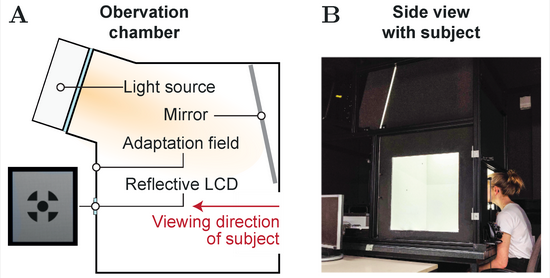
\includegraphics[width=0.6\linewidth]{images/1.png}
    \caption{Экспериментальная установка. (А) Схематическое изображение камеры наблюдения и
    направления обзора. (B) Изображение камеры наблюдения с видом сбоку (дверь для
    обслуживания снята), на котором изображен объект, фокусирующий цель фиксации, которая
    отображается на отражающем жидкокристаллическом дисплее, встроенном в центр задней стенки
    камеры. Подставка для подбородка используется для соответствующего позиционирования и
    выравнивания головы субъекта.\cite{sternberg_paradigm}}
    \label{fig_1}
\end{figure}

Парадигма Стернберга была успешно использована в рамках изучения индивидуальных различий в
процессах памяти у здоровых участников \cite{paradigm_1}, \cite{paradigm_2}, в
исследованиях посвященных изучению дефицитарности и изменений кратковременной памяти при
старении \cite{paradigm_3}, в исследованиях шизофрении и болезни
Альцгеймера \cite{paradigm_4}, депрессии \cite{paradigm_5}, множественного склероза \cite{paradigm_6}, в
исследованиях изучающих воздействия различных медикаментов на процессы памяти \cite{paradigm_7}.\\[0.5 cm]

\subsection{Процедура снятия ЭЭГ данных}
\label{sec:chapter_2_2}

\vspace*{10 mm}
В настоящем исследования для получения ЭЭГ данных использовался "Тест Стернберга".
В эксперименте на голову участника исследования одевается специальная шапочка со специальными
металлическими электродами, которые регистрирует биоэлектрическую активность мозга (см. рис.
\ref{fig_2}). Каждый электрод с какой-то частотой (обычно 500-1000 Гц) регистрирует амплитуду
колебаний электромагнитной активности изменения электрического потенциала с поверхности головы. 

\begin{wrapfigure}{r}{0.4\textwidth}
    \centering
    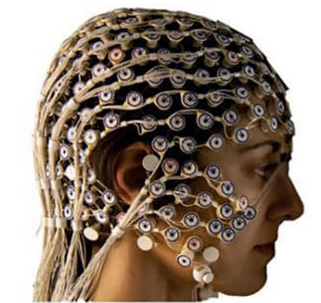
\includegraphics[width=0.4\textwidth]{images/2.png}
    \caption{Расположение электродов на поверхности головы}
    \label{fig_2}
\end{wrapfigure}

Затем участнику эксперимента последовательно предъявляются наборы цифр.
В каждом наборе цифры от 1 до 9 (без повторений одной цифры дважды) были представлены в случайной
последовательности. При этом размеры наборов могут отличаться (в оригинальных исследованиях
Стернберга, как было описано выше, это наборы объемом от 1 до 6 цифр). В зависимости от того,
какой длины последовательность была предъявлена участнику, определялся тип решаемой задачи:
лёгкая, средняя, повышенной сложности и тяжёлая (3, 4, 5 или 6 и более цифр для запоминания
соответственно)--- всего 4 типа задачи. Цифры показываются одна
за другой, участнику необходимо запомнить их последовательность. После контрольного сигнала
(появление определенной цифры на экране) участнику необходимо как можно быстрее ответить,
присутствовала ли цифра в предъявленном до этого наборе. После этого участника просят вспомнить
порядок представления цифр, для того чтобы убедиться, что он действительно запомнил
последовательность.

Перед предъявлением набора стимулов участникам эксперимента предъявляется фиксационный крест
на 1 секунду. Предъявление набора стимулов начинается через 1.2 секунды после предъявления
фиксационного креста и длится 1.5 секунды. Через 2 секунды после окончания предъявления набора
предъявляется тестовый стимул (задача участника - сказать был ли тестовый стимул в наборе).
Тестовый стимул предъявляется на 2 секунды. С момента начала предъявления тестового стимула
участник может давать ответ.

В исследовании принимал участие 101 человек. Каждому человеку предлагалось для решения порядка
30 задач на каждый из 4 типов. %% Использованные данные (как данные снимались)
    \newpage

\section{Формат данных}

\subsection{Проблемы при регистрации ЭЭГ}

После того, как ЭЭГ снято, необходимо отфильтровать сигнал. Сигнал плохо виден
на фоне шума, который создают различные артефакты.  

При регистрации ЭЭГ артефактом является любая активность, не связанная с электрической
активностью мозга. Все артефакты при регистрации ЭЭГ могут быть разделены на две группы:
\begin{enumerate}
    \item артефакты, связанные с аппаратурой, внешние помехи физической природы; 
    \item физиологические артефакты, регистрируемые от больного. 
\end{enumerate}
Наиболее частыми являются артефакты, связанные с регистрацией потенциалов, возникающих при моргании и движении глаз,
миографических потенциалов при мышечном напряжении.  

В связи с этим возникает проблема обработки записи ЭЭГ --- необходимо
удалить артефакты, чтобы получить более точные показатели.

\label{sec:chapter_3_2}
\subsection{Предварительная обработка данных}

Для удаления артефактов был использованный автоматический метод, реализованный для
среды обработки ЭЭГ (MNE) \cite{MNE}. После предварительной очистки данные ЭЭГ были
отфильтрованы в диапазоне частот 1-30 Гц. Далее с помощью метода Уэлча для стандартных
узких частотных диапазонов ЭЭГ
\begin{itemize}
    \item $\delta:\:$ 1-4 Гц
    \item $\theta:\:$ 4-8 Гц
    \item $\alpha_1:\:$ 8-10 Гц
    \item $\alpha_2:\:$ 10-13 Гц
    \item $\beta_1:\:$ 13-20 Гц
    \item $\beta_2:\:$ 20-30 Гц
\end{itemize}
спектральная мощность сигнала была проанализирована отдельно для тестов Стернберга
разной сложности (3, 4, 5 или 6 цифр и более для запоминания).

После удаления артефактов данные были получены в виде набора .csv файлов. Каждый файл содержал
в себе данные, относящиеся к конкретному человеку и типу задачи (см. главу
\ref{sec:chapter_2_2}),то есть всего 404 файла. Данные из файлов были объединены
в один набор данных, пригодных для обработки алгоритмами машинного обучения.

\subsection{Вид полученных данных}
\label{sec:chapter_3_3}

Полученный набор данных устроен следующим образом (см. рис. \ref{fig_3})\\
\begin{figure}[H]
    \centering
    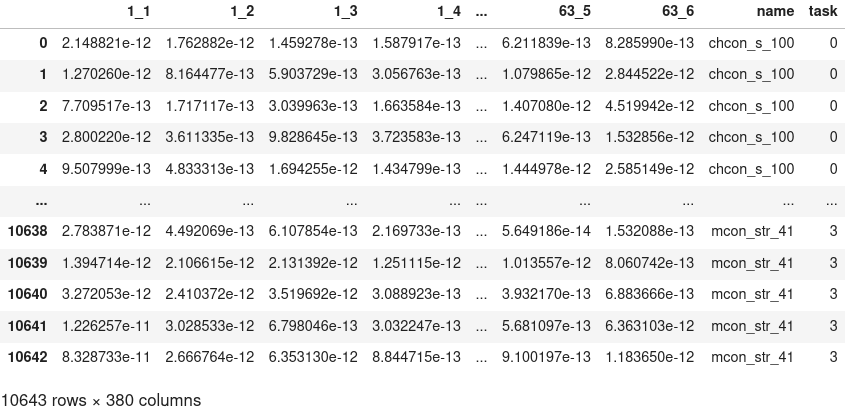
\includegraphics[width=\linewidth]{images/3.png}
    \caption{Полученный набор данных ЭЭГ}
    \label{fig_3}
\end{figure}

Каждая строка нашей выборки имеет размерность $63\cdot 6+1+1=380$. В строке первые $63\cdot 6=378$
ячеек есть амплитуды колебаний электромагнитной активности, которые регистрировались
каждым из 63 электродов (каждый электрод в свою очередь характеризуется шестью частотными
диапазонами спектра). Также есть столбец $"name"$, содержащий идентификатор участника
эксперимента, и столбец $"task"$ с соответствующим типом задачи, которую решал участник во
время снятия ЭЭГ данных. Каждому из 4 типов задачи (лёгкая, средняя, повышенной сложности
и трудная) соответствует число от 0 до 3.

Всего 101 участником эксперимента было решено от 22 до 32 задач каждого из 4 типов сложности.
На каждого человека приходится всего порядка 80--120 задач.
Суммарное количество объектов в выборке составляет 10643.

Рассмотрим объект выборки более подробно (см. рис. \ref{fig_4}):
\begin{itemize}
    \item \textcolor{red}{Красным цветом} выделены амплитуды колебаний электромагнитной
    активности электродов (каждый из 63 характеризуется шестью частотными диапазонами).
    В каждой ячейке значением является вещественное число;
    \item \textcolor{green}{Зелёным цветом} --- идентификатор участника; 
    \item \textcolor{blue}{Синим цветом} --- тип задачи (число от 0 до 3).
\end{itemize}


\begin{figure}[H]
    \centering
    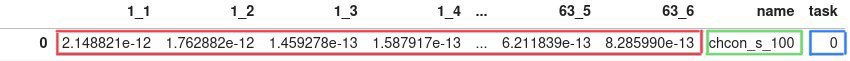
\includegraphics[width=\linewidth]{images/4.png}
    \caption{Детальный вид объекта выборки}
    \label{fig_4}
\end{figure}
 %% Формат данных (как устроены данные)
    \newpage

\section{Постановка задачи}

\subsection{Задача обучения классификатора}

\subsection{Цели и задачи}

\subsection{Выбор метода} %% Предобработка данных \ предварительная обработка
    %\section{Описание практической части}
%\label{sec:Chapter4} \index{Chapter4}
Если в рамках работы писался какой-то код, здесь должно быть его описание: выбранный язык и библиотеки и мотивы выбора, архитектура, схема функционирования, теоретическая сложность алгоритма, характеристики функционирования (скорость/память).

\newpage %% Описание практической части
    %\newpage
\section{Обработка результатов}
%\label{sec:Chapter5} \index{Chapter5}

\subsection{Оценки качества предсказания}

Допустим, что можно получить качество предсказания классификатора свыше 60\%,
рассматривая электроды по отдельности.
% Предположим, что следующая гипотеза истинна: 
% \begin{equation}
%     \label{eq:hypothesis}
%     \begin{aligned}
%         &\text{рассматривая электроды отдельно друг от друга, можно}\\
%         &\text{получить результат (качество предсказания классификатора),}\\
%         &\text{точность которого свыше 60\%.} 
%     \end{aligned}
% \end{equation}
 
Проанализируем полученные данные.\\
В результате применения линейного метода машинного обучения (логистической регрессии)
на обучающих выборках типа (\ref{eq:eq_2}) получаем следующие результаты, которые
изобразим в виде столбчатой диаграммы:

\begin{figure}[H]
    \centering
    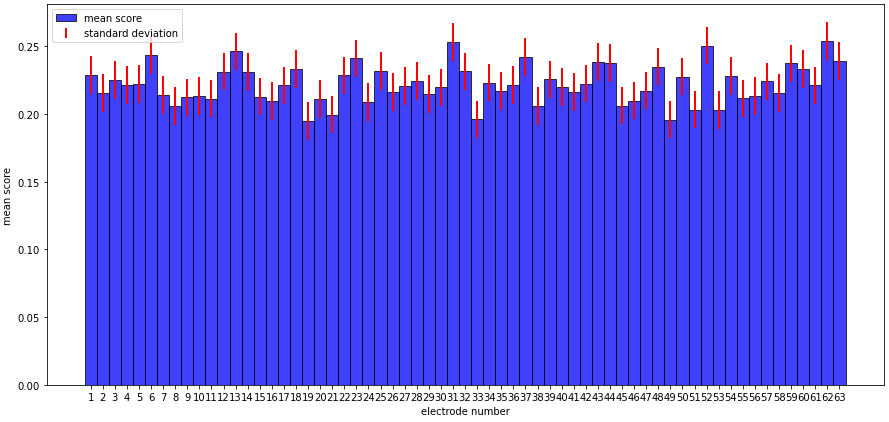
\includegraphics[width=1.05\linewidth]{images/mean_scores.png}
    \caption{Оценки качества предсказания натренированных классификаторов.
    По оси абсцисс --- номера электродов, по оси ординат --- средние по всем участникам
    эксперимента оценки качества предсказания.}
    \label{fig_12}
\end{figure}

Опираясь на изображённую столбчатую диаграмму, можем сформировать представление о том,
как амплитуда биоэлектрической активности, регистрируемой электродом с конкретной зоны
мозга, в отдельности влияет на результат классификации типа решаемой задачи и какие из
них наибольшим образом влияют на результат.

Однако посмотрим на диапазон средних значений оценок качества предсказания
натренированных классификаторов --- варьируется от $\thicksim 0.2$ до $\thicksim 0.25$.
Что интерпретируется следующим образом: доля правильно предсказанных ответов алгоритмом
составляет 20--25\%. Данное утверждение заставляет задуматься о целесообразности
использования в дальнейшем полученных результатов.

Покажем формально, что рассматривать электроды таким образом (то есть по отдельности)
нецелесообразно.

\subsection{P-value}

P-value --- величина, используемая при тестировании статистических гипотез. Фактически
это вероятность ошибки при отклонении нулевой гипотезы (ошибки первого рода) \cite{statistics}.

Пусть $X$ --- множество объектов выборки, $H_0$ --- некоторая нулевая гипотеза, а $T(X)$ --- статистика,
используемая при проверке гипотезы $H_0$. Предполагаем, что если $H_0$ истинна, то распределение
статистики $T(X)$ известно.

Обозначив функцию распределения $F(t)=P(T<t)$, p-value определяется как: $P(t)=2\min(P_{0},P)$.
% % ***********8
% \subsubsection{Формальное определение}

% Пусть есть некоторое значение 
% % здесь подробнее про p-value из wiki
% % ***********

% \begin{figure}[H]
%     \centering
%     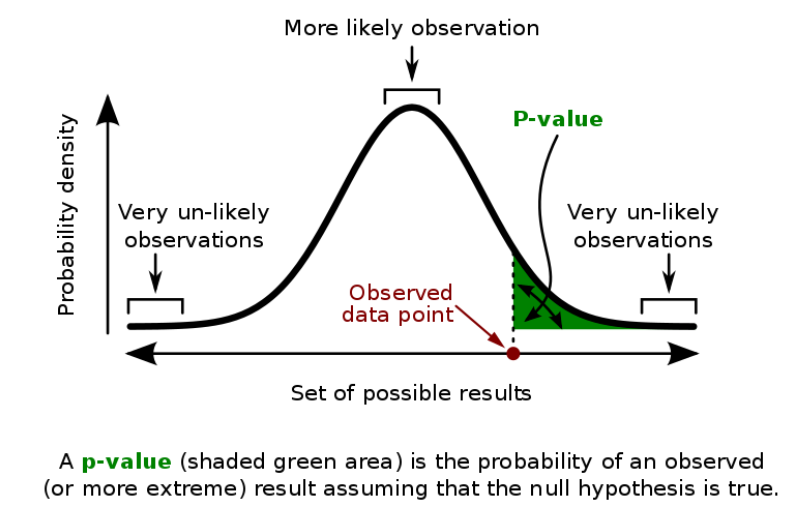
\includegraphics[width=0.8\linewidth]{images/pvalue.png}
%     \caption{Пример вычисления p-value. Вертикальная координата — плотность вероятности
%     каждого результата, вычисленная для нулевой гипотезы. Величина p-value — область под
%     кривой, ограниченной по оси абсцисс наблюдаемой точкой данных.}
%     \label{pvalue}
% \end{figure}


\subsubsection{Применение к логистической регрессии}
\label{sec:chapter_6_2}

Когда мы используем логистическую регрессию, мы используем некоторые независимые
переменные для прогнозирования зависимой переменной (см. главу \ref{sec:chapter_5_2}).
Таким образом, применяя логистическую регрессию, мы получаем коэффициенты для каждой
независимой переменной, которые мы использовали для прогнозирования зависимой переменной.

Рассматривая нашу нулевую гипотезу (cм. главу \ref{sec:hypothesis}) мы предполагаем, что
нет корреляции между признаками и целевыми переменными. В логистической регрессии мы предполагаем, что используемая независимая переменная
(признак) является статистически незначимой (т.е. нет корреляции между признаками
и целевыми переменными) для прогнозирования зависимой переменной или, проще говоря,
её коэффициент корреляции будет равен 0.

Поэтому чем меньше p-value, тем более статистически значимой является рассматриваемая переменная
для нашей модели логистической регрессии.

Допустим, мы получили p-value равное 0.03 или 3\%. Тогда это означает что наши результаты
случайны лишь на 3\% и на столько же не зависят от данного эксперимента. Поэтому, если получим
p-value < 5\%, то придём к выводу, что переменная является значимой и отвергнем нашу
нулевую гипотезу в пользу альтернативной гипотезы.

\subsubsection{Реализация}

Для вычисления p-value воспользовались готовой реализацией statsmodels.
Statsmodels — это python-модуль, который предоставляет классы и функции для оценки
множества различных статистических моделей, а также для проведения статистических тестов
и исследования статистических данных. Для каждой реализации доступен обширный список 
статистики результатов. Результаты проверяются на соответствие существующим статистическим
пакетам, чтобы убедиться в их правильности. Пакет выпущен под лицензией Modified BSD с
открытым исходным кодом \cite{BSD}, \cite{statsmodels}.

\begin{figure}[H]
    \centering
    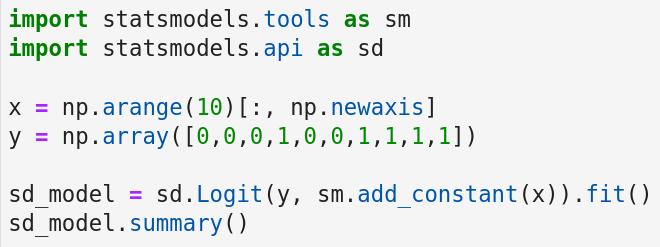
\includegraphics[width=0.7\linewidth]{images/12_2.png}
    \caption{Пример использования готовой реализации для вычисления p-value на языке Python}
    \label{fig_13}
\end{figure}
%
    \let\OriginalVerbatim=\Verbatim
    \makeatletter
    \renewcommand{\Verbatim}[1][1]{%
        %\parskip\z@skip
        \sbox\Wrappedcontinuationbox {\Wrappedcontinuationsymbol}%
        \sbox\Wrappedvisiblespacebox {\FV@SetupFont\Wrappedvisiblespace}%
        \def\FancyVerbFormatLine ##1{\hsize\linewidth
            \vtop{\raggedright\hyphenpenalty\z@\exhyphenpenalty\z@
                \doublehyphendemerits\z@\finalhyphendemerits\z@
                \strut ##1\strut}%
        }%
        % If the linebreak is at a space, the latter will be displayed as visible
        % space at end of first line, and a continuation symbol starts next line.
        % Stretch/shrink are however usually zero for typewriter font.
        \def\FV@Space {%
            \nobreak\hskip\z@ plus\fontdimen3\font minus\fontdimen4\font
            \discretionary{\copy\Wrappedvisiblespacebox}{\Wrappedafterbreak}
            {\kern\fontdimen2\font}%
        }%
        
        % Allow breaks at special characters using \PYG... macros.
        \Wrappedbreaksatspecials
        % Breaks at punctuation characters . , ; ? ! and / need catcode=\active 	
        \OriginalVerbatim[#1,codes*=\Wrappedbreaksatpunct]%
    }
    \makeatother

    % Exact colors from NB
    \definecolor{incolor}{HTML}{303F9F}
    \definecolor{outcolor}{HTML}{D84315}
    \definecolor{cellborder}{HTML}{CFCFCF}
    \definecolor{cellbackground}{HTML}{F7F7F7}
    
    % prompt
    \makeatletter
    \newcommand{\boxspacing}{\kern\kvtcb@left@rule\kern\kvtcb@boxsep}
    \makeatother
    \newcommand{\prompt}[4]{
        {\ttfamily\llap{{\color{#2}[#3]:\hspace{3pt}#4}}\vspace{-\baselineskip}}
    }
    

    
    % Prevent overflowing lines due to hard-to-break entities
    \sloppy 
    % Setup hyperref package
    \hypersetup{
      breaklinks=true,  % so long urls are correctly broken across lines
      colorlinks=true,
      urlcolor=urlcolor,
      linkcolor=linkcolor,
      citecolor=citecolor,
      }
    % Slightly bigger margins than the latex defaults
    
    \geometry{verbose,tmargin=1in,bmargin=1in,lmargin=1in,rmargin=1in}
    
    

\begin{document}
    
    \maketitle
    
    

    
    \begin{tcolorbox}[breakable, size=fbox, boxrule=1pt, pad at break*=1mm,colback=cellbackground, colframe=cellborder]
\prompt{In}{incolor}{1}{\boxspacing}
\begin{Verbatim}[commandchars=\\\{\}]
\PY{k+kn}{import} \PY{n+nn}{numpy} \PY{k}{as} \PY{n+nn}{np}
\PY{k+kn}{from} \PY{n+nn}{scipy}\PY{n+nn}{.}\PY{n+nn}{stats} \PY{k+kn}{import} \PY{n}{norm}
\PY{k+kn}{from} \PY{n+nn}{sklearn}\PY{n+nn}{.}\PY{n+nn}{linear\PYZus{}model} \PY{k+kn}{import} \PY{n}{LogisticRegression}

\PY{k}{def} \PY{n+nf}{logit\PYZus{}pvalue}\PY{p}{(}\PY{n}{model}\PY{p}{,} \PY{n}{x}\PY{p}{)}\PY{p}{:}
    \PY{n}{p1} \PY{o}{=} \PY{n}{model}\PY{o}{.}\PY{n}{predict\PYZus{}proba}\PY{p}{(}\PY{n}{x}\PY{p}{)}
    \PY{n}{n1} \PY{o}{=} \PY{n+nb}{len}\PY{p}{(}\PY{n}{p1}\PY{p}{)}
    \PY{n}{m1} \PY{o}{=} \PY{n+nb}{len}\PY{p}{(}\PY{n}{model}\PY{o}{.}\PY{n}{coef\PYZus{}}\PY{p}{[}\PY{l+m+mi}{0}\PY{p}{]}\PY{p}{)} \PY{o}{+} \PY{l+m+mi}{1}
    \PY{n}{coefs} \PY{o}{=} \PY{n}{np}\PY{o}{.}\PY{n}{concatenate}\PY{p}{(}\PY{p}{[}\PY{n}{model}\PY{o}{.}\PY{n}{intercept\PYZus{}}\PY{p}{,} \PY{n}{model}\PY{o}{.}\PY{n}{coef\PYZus{}}\PY{p}{[}\PY{l+m+mi}{0}\PY{p}{]}\PY{p}{]}\PY{p}{)}
    \PY{n}{x\PYZus{}full} \PY{o}{=} \PY{n}{np}\PY{o}{.}\PY{n}{matrix}\PY{p}{(}\PY{n}{np}\PY{o}{.}\PY{n}{insert}\PY{p}{(}\PY{n}{np}\PY{o}{.}\PY{n}{array}\PY{p}{(}\PY{n}{x}\PY{p}{)}\PY{p}{,} \PY{l+m+mi}{0}\PY{p}{,} \PY{l+m+mi}{1}\PY{p}{,} \PY{n}{axis} \PY{o}{=} \PY{l+m+mi}{1}\PY{p}{)}\PY{p}{)}
    \PY{n}{answ} \PY{o}{=} \PY{n}{np}\PY{o}{.}\PY{n}{zeros}\PY{p}{(}\PY{p}{(}\PY{n}{m1}\PY{p}{,} \PY{n}{m1}\PY{p}{)}\PY{p}{)}
    \PY{k}{for} \PY{n}{i} \PY{o+ow}{in} \PY{n+nb}{range}\PY{p}{(}\PY{n}{n1}\PY{p}{)}\PY{p}{:}
        \PY{n}{answ} \PY{o}{=} \PY{n}{answ} \PYZbs{}
            \PY{o}{+} \PY{n}{np}\PY{o}{.}\PY{n}{dot}\PY{p}{(}\PY{n}{np}\PY{o}{.}\PY{n}{transpose}\PY{p}{(}\PY{n}{x\PYZus{}full}\PY{p}{[}\PY{n}{i}\PY{p}{,} \PY{p}{:}\PY{p}{]}\PY{p}{)}\PY{p}{,} \PY{n}{x\PYZus{}full}\PY{p}{[}\PY{n}{i}\PY{p}{,} \PY{p}{:}\PY{p}{]}\PY{p}{)} \PYZbs{}
            \PY{o}{*} \PY{n}{p1}\PY{p}{[}\PY{n}{i}\PY{p}{,}\PY{l+m+mi}{1}\PY{p}{]} \PY{o}{*} \PY{n}{p1}\PY{p}{[}\PY{n}{i}\PY{p}{,} \PY{l+m+mi}{0}\PY{p}{]}
    \PY{n}{vcov} \PY{o}{=} \PY{n}{np}\PY{o}{.}\PY{n}{linalg}\PY{o}{.}\PY{n}{inv}\PY{p}{(}\PY{n}{np}\PY{o}{.}\PY{n}{matrix}\PY{p}{(}\PY{n}{answ}\PY{p}{)}\PY{p}{)}
    \PY{n}{se} \PY{o}{=} \PY{n}{np}\PY{o}{.}\PY{n}{sqrt}\PY{p}{(}\PY{n}{np}\PY{o}{.}\PY{n}{diag}\PY{p}{(}\PY{n}{vcov}\PY{p}{)}\PY{p}{)}
    \PY{n}{t1} \PY{o}{=}  \PY{n}{coefs}\PY{o}{/}\PY{n}{se}  
    \PY{n}{p1} \PY{o}{=} \PY{p}{(}\PY{l+m+mi}{1} \PY{o}{\PYZhy{}} \PY{n}{norm}\PY{o}{.}\PY{n}{cdf}\PY{p}{(}\PY{n+nb}{abs}\PY{p}{(}\PY{n}{t1}\PY{p}{)}\PY{p}{)}\PY{p}{)} \PY{o}{*} \PY{l+m+mi}{2}
    \PY{k}{return} \PY{n}{p1}

\PY{n}{x} \PY{o}{=} \PY{n}{np}\PY{o}{.}\PY{n}{arange}\PY{p}{(}\PY{l+m+mi}{10}\PY{p}{)}\PY{p}{[}\PY{p}{:}\PY{p}{,} \PY{n}{np}\PY{o}{.}\PY{n}{newaxis}\PY{p}{]}
\PY{n}{y} \PY{o}{=} \PY{n}{np}\PY{o}{.}\PY{n}{array}\PY{p}{(}\PY{p}{[}\PY{l+m+mi}{0}\PY{p}{,}\PY{l+m+mi}{0}\PY{p}{,}\PY{l+m+mi}{0}\PY{p}{,}\PY{l+m+mi}{1}\PY{p}{,}\PY{l+m+mi}{0}\PY{p}{,}\PY{l+m+mi}{0}\PY{p}{,}\PY{l+m+mi}{1}\PY{p}{,}\PY{l+m+mi}{1}\PY{p}{,}\PY{l+m+mi}{1}\PY{p}{,}\PY{l+m+mi}{1}\PY{p}{]}\PY{p}{)}
\PY{n}{model} \PY{o}{=} \PY{n}{LogisticRegression}\PY{p}{(}\PY{n}{C}\PY{o}{=}\PY{l+m+mf}{1e30}\PY{p}{)}\PY{o}{.}\PY{n}{fit}\PY{p}{(}\PY{n}{x}\PY{p}{,} \PY{n}{y}\PY{p}{)}
\PY{n+nb}{print}\PY{p}{(}\PY{n}{logit\PYZus{}pvalue}\PY{p}{(}\PY{n}{model}\PY{p}{,} \PY{n}{x}\PY{p}{)}\PY{p}{)}

\PY{k+kn}{import} \PY{n+nn}{statsmodels}\PY{n+nn}{.}\PY{n+nn}{tools} \PY{k}{as} \PY{n+nn}{sm}
\PY{k+kn}{import} \PY{n+nn}{statsmodels}\PY{n+nn}{.}\PY{n+nn}{api} \PY{k}{as} \PY{n+nn}{sd}
\PY{n}{sd\PYZus{}model} \PY{o}{=} \PY{n}{sd}\PY{o}{.}\PY{n}{Logit}\PY{p}{(}\PY{n}{y}\PY{p}{,} \PY{n}{sm}\PY{o}{.}\PY{n}{add\PYZus{}constant}\PY{p}{(}\PY{n}{x}\PY{p}{)}\PY{p}{)}\PY{o}{.}\PY{n}{fit}\PY{p}{(}\PY{n}{disp}\PY{o}{=}\PY{l+m+mi}{0}\PY{p}{)}
\PY{n+nb}{print}\PY{p}{(}\PY{n}{sd\PYZus{}model}\PY{o}{.}\PY{n}{pvalues}\PY{p}{)}
\PY{n}{sd\PYZus{}model}\PY{o}{.}\PY{n}{summary}\PY{p}{(}\PY{p}{)}
\end{Verbatim}
\end{tcolorbox}

    \begin{Verbatim}[commandchars=\\\{\}]
[0.11413069 0.08780009]
[0.11413093 0.08779979]
    \end{Verbatim}

            \begin{tcolorbox}[breakable, size=fbox, boxrule=.5pt, pad at break*=1mm, opacityfill=0]
\prompt{Out}{outcolor}{1}{\boxspacing}
\begin{Verbatim}[commandchars=\\\{\}]
<class 'statsmodels.iolib.summary.Summary'>
"""
                           Logit Regression Results
==============================================================================
Dep. Variable:                      y   No. Observations:                   10
Model:                          Logit   Df Residuals:                        8
Method:                           MLE   Df Model:                            1
Date:                Sun, 19 Jun 2022   Pseudo R-squ.:                  0.4856
Time:                        22:48:10   Log-Likelihood:                -3.5656
converged:                       True   LL-Null:                       -6.9315
Covariance Type:            nonrobust   LLR p-value:                  0.009472
==============================================================================
                 coef    std err          z      P>|z|      [0.025      0.975]
------------------------------------------------------------------------------
const         -3.9587      2.506     -1.580      0.114      -8.870       0.952
x1             0.8797      0.515      1.707      0.088      -0.130       1.890
==============================================================================
"""
\end{Verbatim}
\end{tcolorbox}
        

    % Add a bibliography block to the postdoc
    
    
    
\end{document}


\begin{figure}[H]
    \centering
    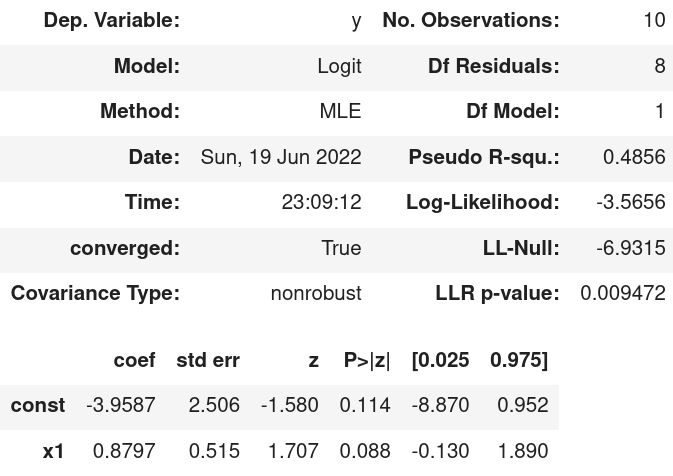
\includegraphics[width=0.7\linewidth]{images/13.png}
    \caption{Вывод работы программы}
    \label{fig_14}
\end{figure}

\subsection{Формулировка гипотезы}

\label{sec:hypothesis}
\begin{flushleft}
    Рассматривая электроды отдельно друг от друга, можно получить результат (качество
    предсказания классификатора), точность которого свыше 60\%.
\end{flushleft} 

% \begin{equation}
%     \label{eq:hypothesis}
%     \begin{aligned}
%         &\text{Рассматривая электроды отдельно друг от друга, можно}\\
%         &\text{получить результат (качество предсказания классификатора),}\\
%         &\text{точность которого свыше 60\%.} 
%     \end{aligned}
% \end{equation}

\subsection{Доказательство}

\subsubsection{Подход №1}
В нашем случае наша гипотеза о том, что с помощью одного электрода можно получить результат,
точность которого больше 60\%
(см. главу\ref{sec:hypothesis}), будет нулевой гипотезой. Тогда альтернативной гипотезой будет 
противоположная ей, о том, что нельзя получить результат с точностью больше 60\%.

Предположим наша нулевая гипотеза истинна. Тогда вычислим p-value для
каждой полученной предсказательной модели. Получим, что максимальное значение по всем
p-value равно 4.8\%, минимальное значение --- 0.7\%, а среднее --- 4.2\% (см. таблицу \ref{fig:table_1}):\\[1 mm]

\begin{table}[H]

    \begin{center}
        \caption{Результаты вычисления p-value}
        \begin{tabular}{ | c | c | c |}
            \hline
            p-value & значение & \% \\ \hline
            max & 0.048 & 4.8\\
            min & 0.007 & 0.7 \\
            mean & 0.042 & 4.2\\
            \hline
        \end{tabular}
        \label{fig:table_1}
    \end{center}
\end{table}

Учитывая, что среднее значение p-value составляет 0.042 или 4.2\%, а p-value каждой модели
не превышает 0.048 или 4.8\% (что меньше 5\%), поэтому мы можем отклонить выдвинутую
гипотезу (нулевую гипотезу) с уровнем значимости 95\% в пользу альтернативной.

\subsubsection{Подход №2}
Используем другой подход. Пусть теперь нулевая гипотеза будет о том, что нельзя получить
точность предсказания классификатора больше 60\%. Вычислим для этого случая p-value.

\begin{table}[H]

    \begin{center}
        \caption{Результаты вычисления p-value}
        \begin{tabular}{ | c | c | c |}
            \hline
            p-value & значение & \% \\ \hline
            max & 0.77 & 77\\
            min & 0.44 & 044 \\
            mean & 0.56 & 56\\
            \hline
        \end{tabular}
        \label{fig:table_2}
    \end{center}
\end{table}

Получив такое p-value нельзя отвергнуть нашу нулевую гипотезу. Данный результат согласуется
с результатом, полученным в предыдущем подходе. Поэтому, рассмотрев несколько подходов, нельзя сказать, что есть хотя бы
один электрод, по которому можно сделать предсказание с точностью свыше 60\%. %% Заключение
    
    \newpage
    %% Don't change the following lines
    \nocite{*}
    \bibliography{references}

    %% в зависимости от надобности подключаем раздел "Приложениие"
    % \newpage
    % \section*{Приложение}
\addcontentsline{toc}{section}{Приложение}
\label{sec:Apendix} \index{Apendix}

Здесь необходимо написать приложение, которое вы должны придумать самомтоятельно
\end{document}